\documentclass{article}
\usepackage[utf8]{inputenc}
\usepackage{graphicx}

\usepackage[english]{babel}
\usepackage{hyperref}
\usepackage[final]{pdfpages}
\usepackage{subfig}
\usepackage{booktabs}
\usepackage{siunitx}
\usepackage{amssymb,amsmath,amsthm}
\usepackage{enumitem}
% Math Script Font
\usepackage{mathrsfs}
% For Indicator Variables
\usepackage{bbold}
% Use \mathscr{}



% Sets the paragraph intends and the paragraph spacing.
\setlength{\parindent}{1em}
\setlength{\parskip}{1em}

% Use the library
\usepackage{natbib}
% Use different spacings
\usepackage{setspace}
% Add package for highlights
\usepackage{color,soul}
% Package for landscape
\usepackage{pdflscape}

% Sets the page margins
\usepackage[margin=1in]{geometry}

% Define some shortcuts
\newcommand{\E}{\mathbb{E}}
\newcommand{\R}{\mathbb{R}}

\newcommand{\figog}[4]{\begin{figure}[h!]\caption{#3}\begin{center}\includegraphics[scale={#1}]{#2}\label{#4}\end{center}\end{figure}}


\def\H{\mathbb{H}}
\DeclareMathOperator{\Log}{log}
\DeclareMathOperator{\Min}{min}
\DeclareMathOperator{\Exp}{exp}
\DeclareMathOperator{\Argmin}{argmin}
\DeclareMathOperator{\Argmax}{argmax}
\DeclareMathOperator{\Sup}{sup}
\DeclareMathOperator{\Inf}{inf}

\def\Argmax#1{\underset{\substack{#1}}{\mbox{argmax }}}
\def\argmax{\mbox{arg}\max}
\def\argmin{\mbox{arg}\min}

% Define NEW environments
\newenvironment{enumog}
	{\begin{enumerate}[noitemsep,topsep=0pt,label*=\arabic*.]}{	\end{enumerate}}

	\newenvironment{itemog}
	{\begin{itemize}[noitemsep,topsep=0pt]}{	\end{itemize}}

\begin{document}

\title{Replication of Angrist et al. 2017}
\author{Oliver Giesecke}

\maketitle 

% NOTE: change system directory first
\begin{table}[h!]
	\begin{center}
		{
\def\sym#1{\ifmmode^{#1}\else\(^{#1}\)\fi}
\begin{tabular}{l*{3}{c}}
\toprule
                &\multicolumn{1}{c}{(1)}         &\multicolumn{1}{c}{(2)}         &\multicolumn{1}{c}{(3)}         \\
\midrule
FFR Expectation &                  &                  &    0.384\sym{***}\\
                &                  &                  & (0.0859)         \\
Inflation, Lag 1&   0.0770         &   0.0488         &   0.0773         \\
                & (0.0733)         & (0.0701)         & (0.0697)         \\
Inflation, Lag 2&                  &   0.0996         &   0.0301         \\
                &                  & (0.0726)         & (0.0698)         \\
Unemployment, Lag 1&   -0.312\sym{***}&   -0.179\sym{**} &   -0.138\sym{*}  \\
                & (0.0955)         & (0.0865)         & (0.0828)         \\
Unemployment, Lag 2&                  &   -0.260\sym{***}&   -0.161\sym{*}  \\
                &                  & (0.0913)         & (0.0835)         \\
Target Rate, Lag 1&                  &  -0.0137\sym{***}&  -0.0208\sym{***}\\
                &                  &(0.00526)         &(0.00587)         \\
Last Change     &                  &   0.0951         &   0.0794         \\
                &                  & (0.0823)         & (0.0787)         \\
FOMC $\times$ Last Change&                  &    0.224\sym{**} &    0.202\sym{**} \\
                &                  &  (0.101)         & (0.0936)         \\
FOMC            &                  &  -0.0283         & -0.00981         \\
                &                  & (0.0312)         & (0.0308)         \\
\midrule
Log-likelihood  &  -187.08         &  -148.81         &  -128.63         \\
Controls        &                  &\checkmark         &\checkmark         \\
Observations    &      192         &      192         &      192         \\
\bottomrule
\end{tabular}
}

	\end{center}
\caption{Replication of Table 1}
\end{table}

Note: Replication of column (1) and (2) seems reasonably accurate. Column (3) which corresponds to model F2 has some discrepancy with respect to the expectation measure that is extracted from federal funds futures. In turn, other estimates also deviate slightly. This needs a little more work.

\begin{figure}
	\begin{center}
			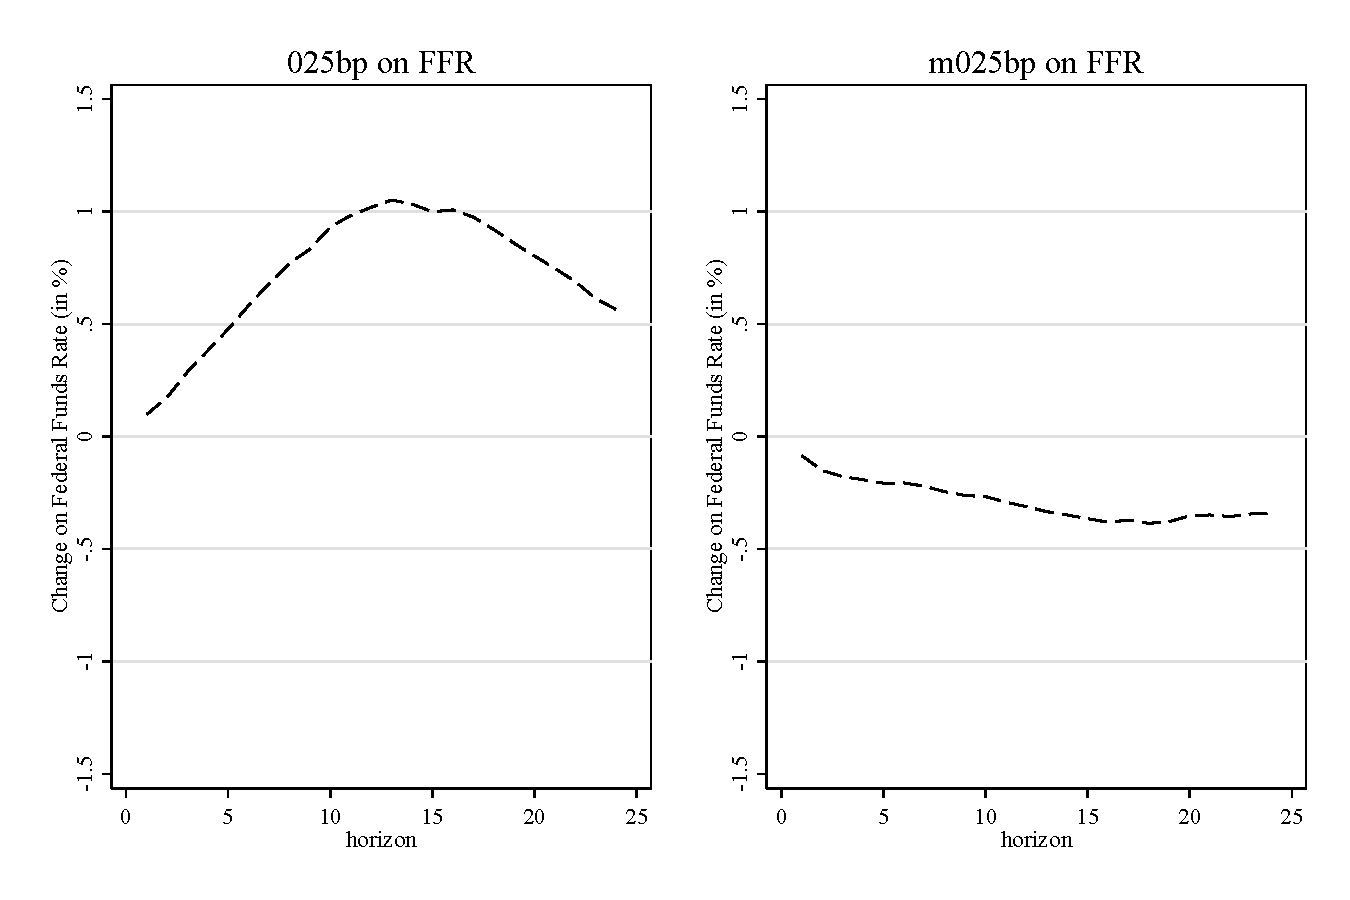
\includegraphics[scale=0.6]{../../output/fig_ffrrate_repl.pdf}
			\caption{Replication Figure 2}
	\end{center}
\end{figure}

\begin{figure}
	\begin{center}
		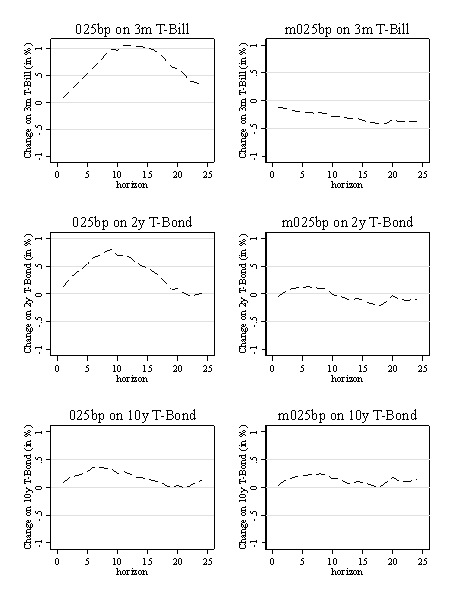
\includegraphics[scale=2]{../../output/fig_tryyields_repl.pdf}
		\caption{Replication Figure 3}
	\end{center}
\end{figure}

\begin{figure}
	\begin{center}
		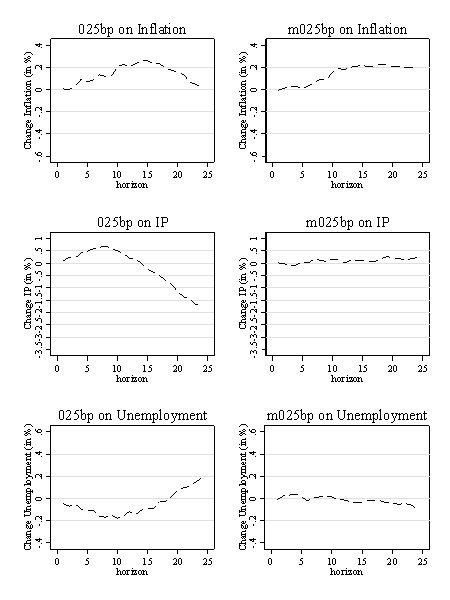
\includegraphics[scale=2]{../../output/fig_realoutcomes_repl.pdf}
		\caption{Replication Figure 4}
	\end{center}
\end{figure}

\end{document}